\documentclass[aspectratio=43]{beamer}

% Keep the Padova theme and all assets local to the thesis project
\makeatletter
\def\input@path{{beamer_padova-0.3/}{thesis/beamer_padova-0.3/}}
\makeatother

\IfFileExists{beamer_padova-0.3/Padova/images/bg.pdf}{%
  \newcommand{\PadovaThemeAssetPath}{beamer_padova-0.3/Padova/images}%
  \newcommand{\ResultPlotPath}{files/runs/batches/thesis_live_30r/chapter3_graphs}%
}{%
  \newcommand{\PadovaThemeAssetPath}{thesis/beamer_padova-0.3/Padova/images}%
  \newcommand{\ResultPlotPath}{thesis/files/runs/batches/thesis_live_30r/chapter3_graphs}%
}

\usetheme{Padova}

\usepackage[utf8]{inputenc}
\usepackage[T1]{fontenc}
\usepackage[english]{babel}
\usepackage{amsmath}
\usepackage{amssymb}
\usepackage{graphicx}
\usepackage{tikz}
\hyphenpenalty=10000
\exhyphenpenalty=10000
\usetikzlibrary{arrows.meta,automata,positioning,calc,fit,backgrounds,shapes.geometric}

\definecolor{unipdRed}{RGB}{180,27,33}
\definecolor{veryPeri}{RGB}{102,102,204}
\definecolor{veryPeriLight}{RGB}{230,230,255}
\definecolor{inkGray}{RGB}{72,79,89}
\definecolor{softGray}{RGB}{244,245,247}
\definecolor{accentTeal}{RGB}{22,142,134}
\definecolor{directBlue}{RGB}{63,109,196}
\definecolor{mediatedOrange}{RGB}{226,112,46}

\setbeamercolor{structure}{fg=unipdRed}
\setbeamercolor{title in head/foot}{fg=white,bg=unipdRed}
\setbeamercolor{author in head/foot}{fg=white,bg=gray!80!black}
\setbeamercolor{date in head/foot}{fg=white,bg=gray!60!black}
\setbeamercolor{evidence box}{fg=inkGray,bg=softGray}
\setbeamercolor{supported panel}{fg=inkGray,bg=accentTeal!7}
\setbeamercolor{boundary panel}{fg=inkGray,bg=unipdRed!6}
\setbeamercolor{title visual}{fg=white,bg=}
\setbeamerfont{caption}{size=\scriptsize}
\setbeamerfont{itemize/enumerate body}{size=\small}
\setbeamerfont{itemize/enumerate subbody}{size=\footnotesize}

\addtobeamertemplate{itemize/enumerate body begin}{%
  \setlength{\itemsep}{0.45em}%
  \setlength{\topsep}{0pt}%
  \setlength{\partopsep}{0pt}%
}{}

\setbeamertemplate{footline}{
  \leavevmode%
  \hbox{%
  \begin{beamercolorbox}[wd=.333333\paperwidth,dp=1.5ex,ht=3ex,center]{author in head/foot}%
    \usebeamerfont{author in head/foot}Alberto Angeloni
  \end{beamercolorbox}%
  \begin{beamercolorbox}[wd=.333333\paperwidth,dp=1.5ex,ht=3ex,center]{title in head/foot}%
    \usebeamerfont{title in head/foot}Gateway Empirical Profiling
  \end{beamercolorbox}%
  \begin{beamercolorbox}[wd=.333333\paperwidth,dp=1.5ex,ht=3ex,center]{date in head/foot}%
    \usebeamerfont{date in head/foot}\insertframenumber{} of \inserttotalframenumber
  \end{beamercolorbox}}%
  \vskip0pt%
}

\setbeamertemplate{navigation symbols}{}

\tikzset{
  visual node/.style={draw=veryPeri,fill=veryPeriLight,rounded corners=2pt,thick,align=center,text=inkGray,font=\scriptsize,minimum height=8mm},
  visual node red/.style={draw=unipdRed,fill=unipdRed!8,rounded corners=2pt,thick,align=center,text=inkGray,font=\scriptsize,minimum height=8mm},
  visual node teal/.style={draw=accentTeal,fill=accentTeal!8,rounded corners=2pt,thick,align=center,text=inkGray,font=\scriptsize,minimum height=8mm},
  visual arrow/.style={-{Stealth[length=2.2mm]},thick,draw=inkGray},
  visual arrow red/.style={-{Stealth[length=2.2mm]},thick,draw=unipdRed},
  visual arrow teal/.style={-{Stealth[length=2.2mm]},thick,draw=accentTeal},
  metric/.style={circle,draw=veryPeri,fill=veryPeriLight,thick,align=center,text=inkGray,font=\scriptsize,minimum size=13mm},
  terminal/.style={circle,draw=unipdRed,fill=unipdRed!8,thick,align=center,text=inkGray,font=\scriptsize,minimum size=13mm}
}

% Centralised presentation metadata and recurring visual grammar
\newcommand{\presentationdate}{25 September 2026}
\newcommand{\sectionprogress}[1]{\framesubtitle{#1 / 05}}
\newcommand{\visualcaption}[1]{%
  \vskip0.35em%
  {\usebeamerfont{caption}\textcolor{gray}{#1}}%
}
\newcommand{\evidencecard}[3]{%
  \begin{beamercolorbox}[wd=\linewidth,sep=.45ex,rounded=true]{evidence box}%
    {\color{#1}\scriptsize\bfseries #2}\par
    \vspace{0.1em}%
    {\raggedright\footnotesize #3\par}%
  \end{beamercolorbox}%
  \vspace{0.22em}%
}

\title{Empirical Profiling of Cloud-Based Healthcare Interoperability Gateways}
\subtitle{Master's Thesis Presentation}
\author{Alberto Angeloni}
\institute{University of Padua}
\date{\presentationdate}

\begin{document}

% Slide 1
\begin{frame}[plain]
  \framesubtitle{00 / 05}
  \vspace{-3mm}
  \begin{columns}[c,totalwidth=.88\paperwidth]
    \begin{column}{.56\paperwidth}
      {\color{white}\Large\bfseries\inserttitle\par}
      \vspace{0.8em}
      {\color{white}\normalsize\insertsubtitle\par}
      \vspace{1.2em}
      {\color{white}\normalsize Alberto Angeloni\par}
      \vspace{0.45em}
      {\color{white}\small University of Padua\par}
      {\color{white}\small Academic Year 2025--2026\par}
      {\color{white}\small\presentationdate\par}
    \end{column}
    \begin{column}{.25\paperwidth}
      \begin{beamercolorbox}[wd=\linewidth,sep=1.1ex,rounded=true,center]{title visual}
        
\includegraphics[width=.82\linewidth,height=12mm,keepaspectratio]{files/img/Logo-UniPD.png}\par
        \vspace{1.1ex}
        
\includegraphics[width=.62\linewidth,height=10mm,keepaspectratio]{files/img/Logo-DM.png}\par
        \vspace{1.1ex}
        
\includegraphics[width=.78\linewidth,height=10mm,keepaspectratio]{files/img/Logo-Informatica-it.png}
      \end{beamercolorbox}
    \end{column}
  \end{columns}
\end{frame}


% Slide 2
\begin{frame}{Narrative Path}
  % \framesubtitle{00 / 05}
  \centering
  \vspace{1.2em}
  \resizebox{.96\textwidth}{!}{%
    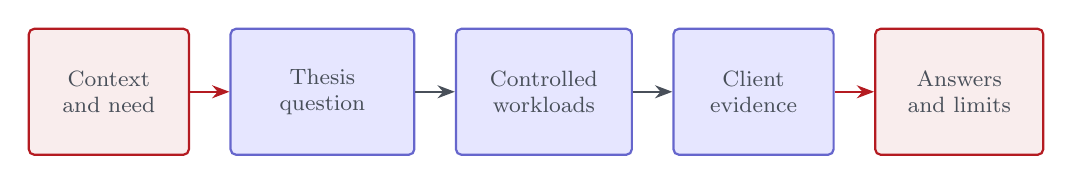
\begin{tikzpicture}[node distance=5mm]
      \node[visual node red,text width=18mm,minimum height=16mm,font=\footnotesize] (context) {Context\\and need};
      \node[visual node,text width=21mm,minimum height=16mm,font=\footnotesize,right=of context] (problem) {Thesis\\question};
      \node[visual node,text width=20mm,minimum height=16mm,font=\footnotesize,right=of problem] (method) {Controlled\\workloads};
      \node[visual node,text width=18mm,minimum height=16mm,font=\footnotesize,right=of method] (evidence) {Client\\evidence};
      \node[visual node red,text width=19mm,minimum height=16mm,font=\footnotesize,right=of evidence] (claims) {Answers\\and limits};
      \draw[visual arrow red] (context) -- (problem);
      \draw[visual arrow] (problem) -- (method);
      \draw[visual arrow] (method) -- (evidence);
      \draw[visual arrow red] (evidence) -- (claims);
    \end{tikzpicture}%
  }
  \vspace{1.7em}
  {\large\color{inkGray}From healthcare needs to defensible conclusions}
\end{frame}

\section{Context and Questions}

% Slide 3
\begin{frame}{Territorial Care Depends on Interoperability}
  \sectionprogress{01}
  \begin{columns}[c,onlytextwidth]
    \begin{column}{.43\textwidth}
      \begin{itemize}
        \item \textbf{Policy} Ministerial Decree 77/2022 reorganises territorial care
        \item \textbf{Transitions} One patient journey spans hospital community and home care
        \item \textbf{Coordination} The Territorial Operations Centre connects care settings
        \item \textbf{Dependency} Care continuity requires timely clinical data exchange
      \end{itemize}
    \end{column}
    \begin{column}{.55\textwidth}
      \centering
      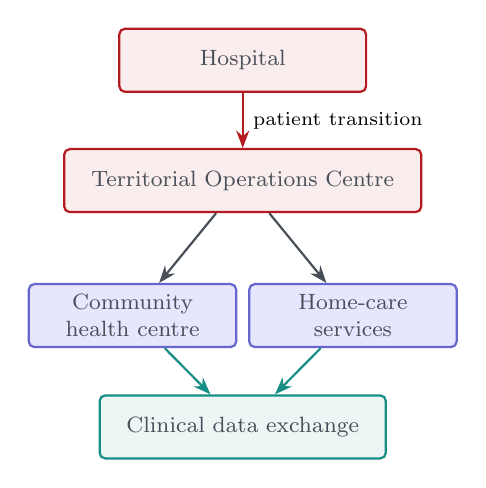
\begin{tikzpicture}[node distance=7mm]
        \node[visual node red,text width=29mm,font=\footnotesize] (hospital) {Hospital};
        \node[visual node red,text width=43mm,font=\footnotesize,below=of hospital] (centre) {Territorial Operations Centre};
        \node[visual node,text width=24mm,font=\footnotesize] (community) at ($(centre.south)+(-14mm,-13mm)$) {Community\\health centre};
        \node[visual node,text width=24mm,font=\footnotesize] (home) at ($(centre.south)+(14mm,-13mm)$) {Home-care\\services};
        \node[visual node teal,text width=34mm,font=\footnotesize] (data) at ($(community.south)!0.5!(home.south)+(0,-10mm)$) {Clinical data exchange};
        \draw[visual arrow red] (hospital) -- node[right,font=\scriptsize] {patient transition} (centre);
        \draw[visual arrow] (centre) -- (community);
        \draw[visual arrow] (centre) -- (home);
        \draw[visual arrow teal] (community) -- (data);
        \draw[visual arrow teal] (home) -- (data);
      \end{tikzpicture}
      \visualcaption{Care transitions depend on a shared information path}
    \end{column}
  \end{columns}
\end{frame}

% Slide 4
\begin{frame}{Thesis Question and Evaluation Lenses}
  \sectionprogress{01}
  \begin{columns}[c,onlytextwidth]
    \begin{column}{.45\textwidth}
      \evidencecard{unipdRed}{PROBLEM}{Endpoint tests alone do not preserve the semantics of an ordered healthcare workflow}
      \vspace{.25em}
      {\scriptsize\bfseries\color{inkGray}THESIS QUESTION}\par
      \vspace{.35em}
      \evidencecard{accentTeal}{WORKLOADS}{How can documented workflows become reproducible end-to-end workloads}
      \evidencecard{veryPeri}{ESTIMATION}{How can apparent mediation overhead be estimated without gateway telemetry}
    \end{column}
    \begin{column}{.53\textwidth}
      \centering
      {\scriptsize\bfseries\color{inkGray}FOUR EVALUATION LENSES}\par
      \vspace{.5em}
      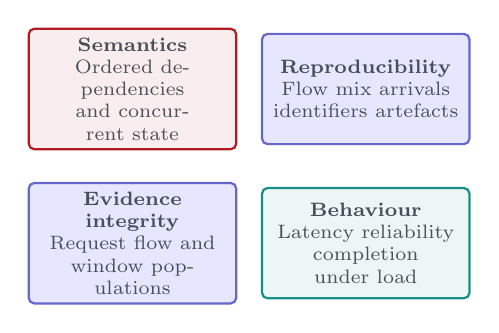
\begin{tikzpicture}[node distance=4mm and 3mm]
        \node[visual node red,text width=24mm,minimum height=14mm] (semantics) {\textbf{Semantics}\\Ordered dependencies\\and concurrent state};
        \node[visual node,text width=24mm,minimum height=14mm,right=of semantics] (repeat) {\textbf{Reproducibility}\\Flow mix arrivals\\identifiers artefacts};
        \node[visual node,text width=24mm,minimum height=14mm,below=of semantics] (integrity) {\textbf{Evidence integrity}\\Request flow and\\window populations};
        \node[visual node teal,text width=24mm,minimum height=14mm,right=of integrity] (behaviour) {\textbf{Behaviour}\\Latency reliability\\completion under load};
      \end{tikzpicture}
      \visualcaption{The lenses operationalise the single thesis question}
    \end{column}
  \end{columns}
\end{frame}

\section{Experimental Method}

% Slide 5
\begin{frame}{Declared Paths Share One Observation Boundary}
  \sectionprogress{02}
  \begin{columns}[c,onlytextwidth]
    \begin{column}{.41\textwidth}
      \evidencecard{unipdRed}{INPUT}{Documented regional workflows}
      \evidencecard{accentTeal}{CONTROL}{Executable occurrences with configured flow mix and arrivals}
      \evidencecard{veryPeri}{COMPARISON}{Declared direct and mediated populations}
      \evidencecard{inkGray}{MEASUREMENT}{Client send-to-response timing and terminal outcomes}
    \end{column}
    \begin{column}{.57\textwidth}
      \centering
      \resizebox{.95\linewidth}{!}{%
      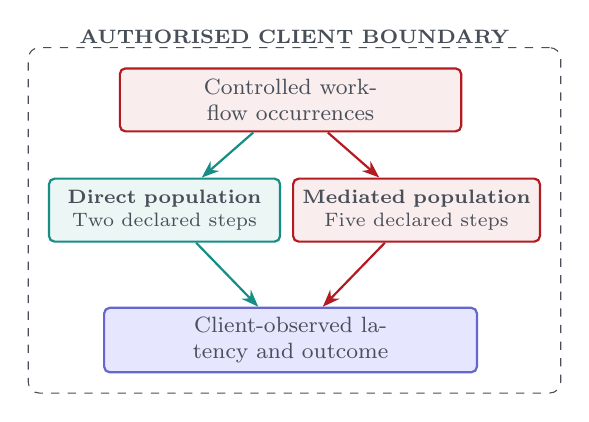
\begin{tikzpicture}
        \node[visual node red,text width=41mm,font=\footnotesize] (workload) at (0,2.25) {Controlled workflow occurrences};
        \node[visual node teal,text width=27mm] (direct) at (-1.6,.85) {\textbf{Direct population}\\Two declared steps};
        \node[visual node red,text width=29mm] (mediated) at (1.6,.85) {\textbf{Mediated population}\\Five declared steps};
        \node[visual node,text width=45mm,font=\footnotesize] (boundary) at (0,-.8) {Client-observed latency and outcome};
        \draw[visual arrow teal] (workload) -- (direct);
        \draw[visual arrow red] (workload) -- (mediated);
        \draw[visual arrow teal] (direct) -- (boundary);
        \draw[visual arrow red] (mediated) -- (boundary);
        \node[draw=inkGray,dashed,rounded corners,fit=(workload)(direct)(mediated)(boundary),inner sep=2.5mm,label={[font=\scriptsize\bfseries,text=inkGray,fill=white,inner sep=1pt]above:AUTHORISED CLIENT BOUNDARY}] {};
      \end{tikzpicture}%
      }
      \visualcaption{The comparison is path-level rather than gateway-only}
    \end{column}
  \end{columns}
\end{frame}

% Slide 6
\begin{frame}{Workflows Produce Traceable Evidence}
  \sectionprogress{02}
  \begin{columns}[c,onlytextwidth]
    \begin{column}{.41\textwidth}
      \evidencecard{accentTeal}{REPRODUCIBILITY CRITERION}{Stable identifiers link configuration workload events and outcomes}
      \evidencecard{unipdRed}{OBSERVED}{All 74 accepted runs retain the complete artefact chain}
      \evidencecard{veryPeri}{CONSISTENCY CHECK}{$757{,}517=2\times299{,}534+158{,}449$}
      \evidencecard{inkGray}{BOUNDARY}{Gateway-internal fields remain empty by design}
    \end{column}
    \begin{column}{.57\textwidth}
      \centering
      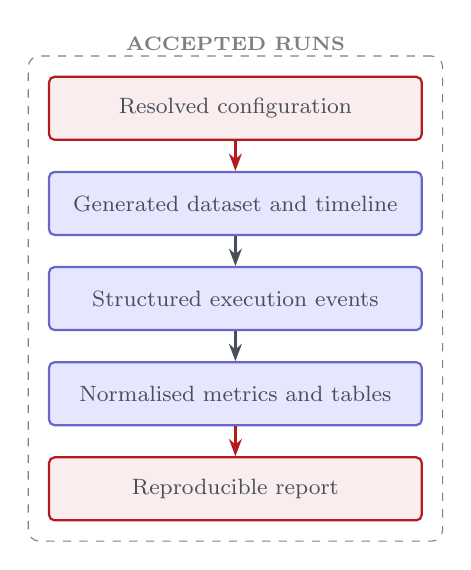
\begin{tikzpicture}[node distance=3.8mm]
        \node[visual node red,text width=45mm,font=\footnotesize] (config) {Resolved configuration};
        \node[visual node,text width=45mm,font=\footnotesize,below=of config] (workload) {Generated dataset and timeline};
        \node[visual node,text width=45mm,font=\footnotesize,below=of workload] (events) {Structured execution events};
        \node[visual node,text width=45mm,font=\footnotesize,below=of events] (metrics) {Normalised metrics and tables};
        \node[visual node red,text width=45mm,font=\footnotesize,below=of metrics] (report) {Reproducible report};
        \draw[visual arrow red] (config) -- (workload);
        \draw[visual arrow] (workload) -- (events);
        \draw[visual arrow] (events) -- (metrics);
        \draw[visual arrow red] (metrics) -- (report);
        \node[draw=gray,dashed,rounded corners,fit=(config)(workload)(events)(metrics)(report),inner sep=2.5mm] {};
        \node[font=\scriptsize\bfseries,text=gray,above=2mm of config] {ACCEPTED RUNS};
      \end{tikzpicture}
    \end{column}
  \end{columns}
\end{frame}

% Slide 7
\begin{frame}{The Realised Evidence Is Smaller Than Planned}
  \sectionprogress{02}
  \begin{columns}[c,onlytextwidth]
    \begin{column}{.42\textwidth}
      \evidencecard{veryPeri}{PLANNED}{300 campaign runs}
      \evidencecard{accentTeal}{STARTED}{145 runs with execution evidence}
      \evidencecard{unipdRed}{COMPLETE}{74 accepted runs across ten scenarios}
      \evidencecard{inkGray}{LIMIT}{Incomplete protocol and unbalanced repetitions support descriptive rather than population-wide claims}
    \end{column}
    \begin{column}{.56\textwidth}
      \centering
      \resizebox{.92\linewidth}{!}{%
        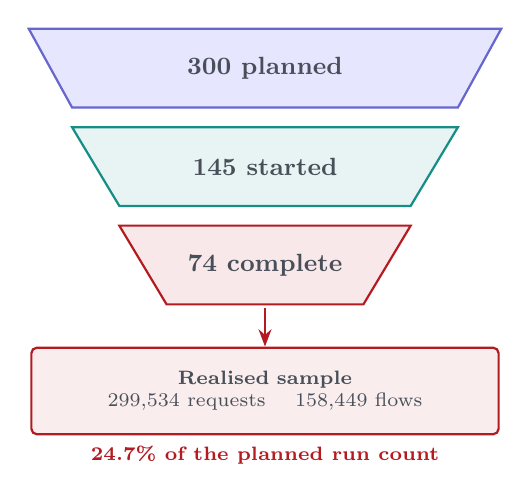
\begin{tikzpicture}[font=\scriptsize]
          \filldraw[fill=veryPeriLight,draw=veryPeri,thick] (-3,3.7) -- (3,3.7) -- (2.45,2.7) -- (-2.45,2.7) -- cycle;
          \node[font=\small\bfseries,text=inkGray] at (0,3.2) {300 planned};
          \filldraw[fill=accentTeal!10,draw=accentTeal,thick] (-2.45,2.45) -- (2.45,2.45) -- (1.85,1.45) -- (-1.85,1.45) -- cycle;
          \node[font=\small\bfseries,text=inkGray] at (0,1.95) {145 started};
          \filldraw[fill=unipdRed!10,draw=unipdRed,thick] (-1.85,1.2) -- (1.85,1.2) -- (1.25,.2) -- (-1.25,.2) -- cycle;
          \node[font=\small\bfseries,text=inkGray] at (0,.7) {74 complete};
          \node[visual node red,text width=57mm,minimum height=11mm] (corpus) at (0,-.9) {\textbf{Realised sample}\\299,534 requests \quad 158,449 flows};
          \draw[visual arrow red] (0,.15) -- (corpus.north);
          \node[font=\scriptsize\bfseries,text=unipdRed] at (0,-1.72) {24.7\% of the planned run count};
        \end{tikzpicture}%
      }
    \end{column}
  \end{columns}
\end{frame}

\section{Empirical Evidence}

% Slide 8
\begin{frame}{Successful-Flow Median Displacement}
  \sectionprogress{03}
  \begin{columns}[c,onlytextwidth]
    \begin{column}{.43\textwidth}
      \evidencecard{accentTeal}{EXPECTED}{Mediated P50 exceeds direct P50 for successful flows}
      \evidencecard{unipdRed}{OBSERVED}{$571.1\,\mathrm{ms}$ direct and $755.8\,\mathrm{ms}$ mediated with $\Delta P_{50}=+184.7\,\mathrm{ms}$}
      \evidencecard{veryPeri}{INTERPRETATION}{Positive client-observed path displacement}
      % \evidencecard{inkGray}{LIMIT}{Two-step and five-step contracts prevent gateway-only attribution}
    \end{column}
    \begin{column}{.55\textwidth}
      \centering
      \begin{tikzpicture}
        \path[use as bounding box] (0,0) rectangle (5.35,5.95);
        \clip (0,0) rectangle (5.35,5.95);
        \node[anchor=south west,inner sep=0] at (0,0) {
\includegraphics[width=10.7cm]{\ResultPlotPath/path_displacement_by_outcome.png}};
      \end{tikzpicture}
      \visualcaption{Empirical successful-flow distributions at the client boundary}
    \end{column}
  \end{columns}
\end{frame}

% Slide 9
\begin{frame}{Early Failure Truncates the Flow Prefix}
  \sectionprogress{03}
  \begin{columns}[c,onlytextwidth]
    \begin{column}{.43\textwidth}
      \evidencecard{accentTeal}{EXPECTED}{An unsuccessful transition suppresses its dependent suffix}
      \evidencecard{unipdRed}{OBSERVED}{$+12.88\,\mathrm{ms}$ failed versus $+184.7\,\mathrm{ms}$ successful}
      \evidencecard{veryPeri}{INTERPRETATION}{The smaller gap is consistent with a shorter realised prefix}
      \evidencecard{inkGray}{LIMIT}{$12.88\,\mathrm{ms}$ is a path differential rather than a failure duration}
    \end{column}
    \begin{column}{.55\textwidth}
      \centering
      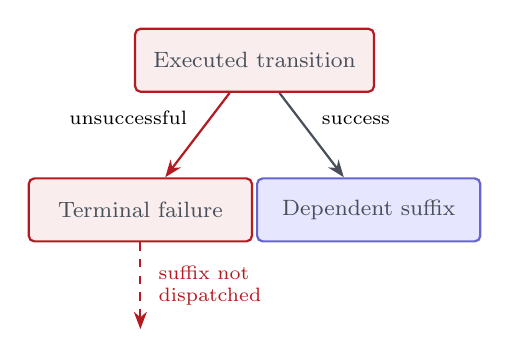
\begin{tikzpicture}
        \node[visual node red,text width=28mm,font=\footnotesize] (executed) at (0,1.55) {Executed transition};
        \node[visual node red,text width=26mm,font=\footnotesize] (failure) at (-1.45,-.35) {Terminal failure};
        \node[visual node,text width=26mm,font=\footnotesize] (suffix) at (1.45,-.35) {Dependent suffix};
        \coordinate (blocked) at ($(failure.south)+(0,-11mm)$);
        \draw[visual arrow] (executed) -- node[above right,font=\scriptsize] {success} (suffix);
        \draw[visual arrow red] (executed) -- node[above left,font=\scriptsize] {unsuccessful} (failure);
        \draw[visual arrow red,dashed] (failure.south) -- node[midway,right=1mm,align=left,font=\scriptsize,text=unipdRed] {suffix not\\dispatched} (blocked);
      \end{tikzpicture}
      \visualcaption{Only executed transitions contribute to the realised prefix}
    \end{column}
  \end{columns}
\end{frame}

% Slide 10
\begin{frame}{Admission Saturation Precedes Delay Growth}
  \sectionprogress{03}
  \begin{columns}[c,onlytextwidth]
    \begin{column}{.40\textwidth}
      \evidencecard{accentTeal}{DESIGN BOUND}{Active client flows $\leq C_{\max}=30$}
      \evidencecard{unipdRed}{OBSERVED}{At $t\approx60\,\mathrm{s}$ active flows reach 30 while P95 queue delay later approaches $67\,\mathrm{s}$}
      \evidencecard{veryPeri}{INTERPRETATION}{Queued occurrences create client-side backpressure}
      \evidencecard{inkGray}{LIMIT}{The plateau does not measure regional gateway capacity}
    \end{column}
    \begin{column}{.58\textwidth}
      \centering
      \resizebox{.92\linewidth}{!}{%
      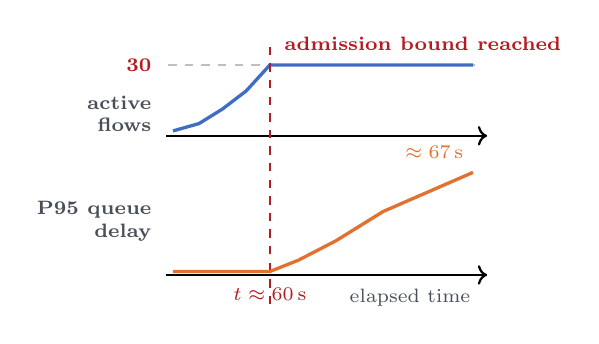
\begin{tikzpicture}[x=.60cm,y=.62cm,font=\scriptsize]
        \draw[->,thick] (.45,3.8) -- (7.25,3.8);
        \node[anchor=east,align=right,font=\scriptsize\bfseries,text=inkGray] at (.35,4.25) {active\\flows};
        \draw[gray!50,dashed] (.5,5.25) -- (7.0,5.25);
        \node[anchor=east,font=\scriptsize\bfseries,text=unipdRed] at (.35,5.25) {30};
        \draw[very thick,directBlue] (.6,3.9) -- (1.15,4.05) -- (1.65,4.35) -- (2.15,4.72) -- (2.65,5.25) -- (6.95,5.25);
        \draw[dashed,unipdRed,thick] (2.65,.35) -- (2.65,5.65);
        \node[anchor=south west,font=\scriptsize\bfseries,text=unipdRed] at (2.75,5.35) {admission bound reached};
        \draw[->,thick] (.45,.95) -- (7.25,.95);
        \node[anchor=east,align=right,font=\scriptsize\bfseries,text=inkGray] at (.35,2.05) {P95 queue\\delay};
        \draw[very thick,mediatedOrange] (.6,1.02) -- (2.65,1.02) -- (3.25,1.25) -- (4.05,1.65) -- (5.05,2.25) -- (6.95,3.05);
        \node[anchor=south east,font=\scriptsize\bfseries,text=mediatedOrange] at (6.95,3.12) {$\approx67\,\mathrm{s}$};
        \node[anchor=north,font=\scriptsize\bfseries,text=unipdRed] at (2.65,.88) {$t\approx60\,\mathrm{s}$};
        \node[anchor=north east,font=\scriptsize,text=inkGray] at (7.1,.86) {elapsed time};
      \end{tikzpicture}%
      }
    \end{column}
  \end{columns}
\end{frame}

% Slide 11
\begin{frame}{Extreme Load Deforms the Latency Distribution}
  \sectionprogress{03}
  \begin{columns}[c,onlytextwidth]
    \begin{column}{.42\textwidth}
      \evidencecard{accentTeal}{EXPECTED}{Successful-flow distribution under extreme versus baseline load}
      \evidencecard{unipdRed}{OBSERVED}{$\mathrm{P50}\ +13.45\%\qquad \mathrm{P95}\ +85.44\%$\\$\mathrm{P99}\ +17.70\%$}
      \evidencecard{veryPeri}{COMPLETION}{Flow success decreases by $3.63$ percentage points}
      \evidencecard{inkGray}{INTERPRETATION}{The upper-tail shoulder changes most}
    \end{column}
    \begin{column}{.56\textwidth}
      \centering
      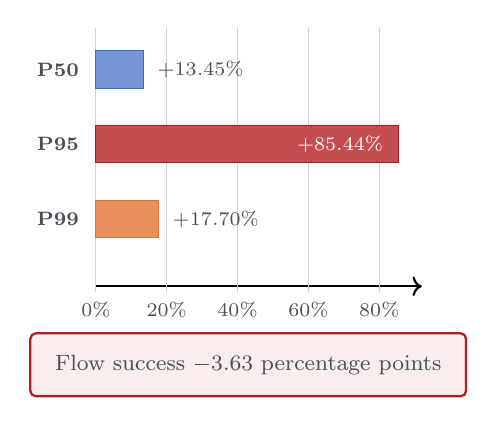
\begin{tikzpicture}[x=.045cm,y=.95cm,font=\scriptsize]
        \draw[->,thick] (0,0) -- (92,0);
        \foreach \x in {0,20,40,60,80} {
          \draw[gray!35] (\x,-.08) -- (\x,3.45);
          \node[anchor=north,text=inkGray] at (\x,-.08) {\x\%};
        }
        \node[anchor=east,font=\scriptsize\bfseries,text=inkGray] at (-2,2.9) {P50};
        \node[anchor=east,font=\scriptsize\bfseries,text=inkGray] at (-2,1.9) {P95};
        \node[anchor=east,font=\scriptsize\bfseries,text=inkGray] at (-2,.9) {P99};
        \filldraw[fill=directBlue!72,draw=directBlue] (0,2.65) rectangle (13.45,3.15);
        \filldraw[fill=unipdRed!78,draw=unipdRed] (0,1.65) rectangle (85.44,2.15);
        \filldraw[fill=mediatedOrange!78,draw=mediatedOrange] (0,.65) rectangle (17.70,1.15);
        \node[anchor=west,font=\scriptsize\bfseries,text=inkGray] at (14.7,2.9) {$+13.45\%$};
        \node[anchor=east,font=\scriptsize\bfseries,text=white] at (83.8,1.9) {$+85.44\%$};
        \node[anchor=west,font=\scriptsize\bfseries,text=inkGray] at (19,.9) {$+17.70\%$};
        \node[visual node red,text width=53mm,font=\footnotesize] at (43,-1.05) {Flow success $-3.63$ percentage points};
      \end{tikzpicture}
      \visualcaption{Extreme stress relative to the baseline constant scenario}
    \end{column}
  \end{columns}
\end{frame}

\section{Claim Boundaries}

% Slide 12
\begin{frame}{Supported Claims and Evidential Boundaries}
  \sectionprogress{04}
  \begin{columns}[T,onlytextwidth]
    \begin{column}{.455\textwidth}
      \begin{beamercolorbox}[wd=\linewidth,sep=.8ex,rounded=true]{supported panel}
        {\normalsize\bfseries\color{accentTeal}SUPPORTED}\par
        \vspace{.3em}
        {\scriptsize\bfseries\color{accentTeal}PATH CHARACTERISATION}\par
        {\footnotesize Client-observed distributions and path-level differentials}\par
        \vspace{.4em}
        {\scriptsize\bfseries\color{accentTeal}WORKFLOW BEHAVIOUR}\par
        {\footnotesize Fail-fast suffix suppression and terminal outcomes}\par
        \vspace{.4em}
        {\scriptsize\bfseries\color{accentTeal}INSTRUMENT LIMIT}\par
        {\footnotesize Client backpressure after the configured bound}\par
      \end{beamercolorbox}
    \end{column}
    \begin{column}{.455\textwidth}
      \begin{beamercolorbox}[wd=\linewidth,sep=.8ex,rounded=true]{boundary panel}
        {\normalsize\bfseries\color{unipdRed}NOT ESTABLISHED}\par
        \vspace{.3em}
        {\scriptsize\bfseries\color{unipdRed}INTERNAL CAUSALITY}\par
        {\footnotesize Gateway-only processing time}\par
        \vspace{.4em}
        {\scriptsize\bfseries\color{unipdRed}REMOTE CAPACITY}\par
        {\footnotesize Provider capacity or a service-level guarantee}\par
        \vspace{.4em}
        {\scriptsize\bfseries\color{unipdRed}GENERALISATION}\par
        {\footnotesize Production-wide traffic representativeness}\par
      \end{beamercolorbox}
    \end{column}
  \end{columns}
  \vspace{.4em}
  \centering
  \begin{beamercolorbox}[wd=.94\textwidth,sep=.45ex,rounded=true,center]{evidence box}
    {\scriptsize\bfseries\color{inkGray}74 complete runs \quad unbalanced repetitions \quad unequal path composition}
  \end{beamercolorbox}
\end{frame}

% Slide 13
\begin{frame}{The Thesis Delivers a Bounded Empirical Profile}
  \sectionprogress{04}
  \begin{columns}[c,onlytextwidth]
    \begin{column}{.44\textwidth}
      \evidencecard{unipdRed}{EXECUTABLE MODEL}{Ordered healthcare workflows become controlled occurrences}
      \evidencecard{accentTeal}{EVIDENCE MODEL}{Identifiers join configuration events requests flows and reports}
      \evidencecard{veryPeri}{EMPIRICAL PROFILE}{Path displacement fail-fast behaviour and load-sensitive tails become observable}
      \evidencecard{inkGray}{CLAIM DISCIPLINE}{Every conclusion remains inside the realised client-observed perimeter}
    \end{column}
    \begin{column}{.54\textwidth}
      \centering
      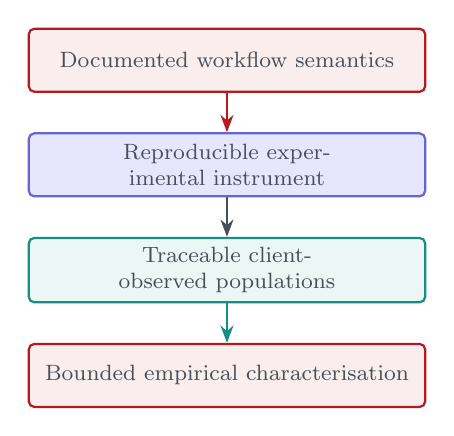
\begin{tikzpicture}[node distance=5mm]
        \node[visual node red,text width=48mm,font=\footnotesize] (workflow) {Documented workflow semantics};
        \node[visual node,text width=48mm,font=\footnotesize,below=of workflow] (instrument) {Reproducible experimental instrument};
        \node[visual node teal,text width=48mm,font=\footnotesize,below=of instrument] (population) {Traceable client-observed populations};
        \node[visual node red,text width=48mm,font=\footnotesize,below=of population] (profile) {Bounded empirical characterisation};
        \draw[visual arrow red] (workflow) -- (instrument);
        \draw[visual arrow] (instrument) -- (population);
        \draw[visual arrow teal] (population) -- (profile);
      \end{tikzpicture}
      \visualcaption{The contribution is the complete chain rather than one isolated metric}
    \end{column}
  \end{columns}
\end{frame}

\section{Conclusions}

% Slide 14
\begin{frame}{Answer to the Thesis Question}
  \sectionprogress{05}
  \centering
  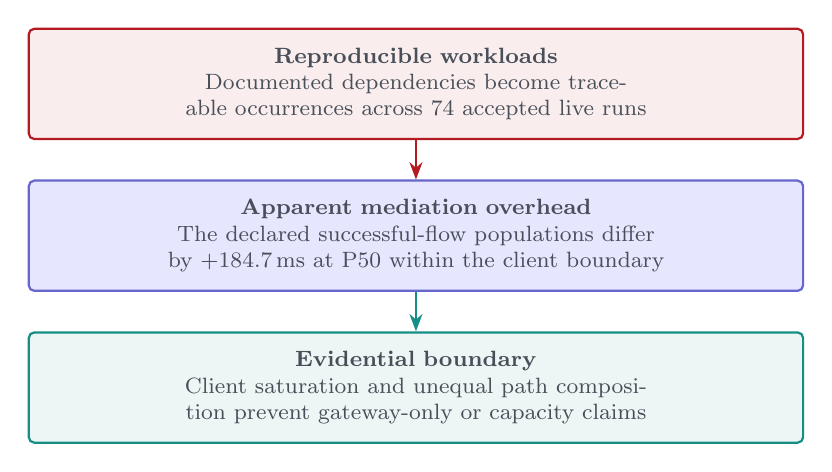
\begin{tikzpicture}[node distance=5mm]
    \node[visual node red,text width=96mm,minimum height=14mm,font=\footnotesize] (workloads) {\textbf{Reproducible workloads}\\Documented dependencies become traceable occurrences across 74 accepted live runs};
    \node[visual node,text width=96mm,minimum height=14mm,font=\footnotesize,below=of workloads] (differential) {\textbf{Apparent mediation overhead}\\The declared successful-flow populations differ by $+184.7\,\mathrm{ms}$ at P50 within the client boundary};
    \node[visual node teal,text width=96mm,minimum height=14mm,font=\footnotesize,below=of differential] (boundary) {\textbf{Evidential boundary}\\Client saturation and unequal path composition prevent gateway-only or capacity claims};
    \draw[visual arrow red] (workloads) -- (differential);
    \draw[visual arrow teal] (differential) -- (boundary);
  \end{tikzpicture}
  \vspace{.35em}
  \begin{beamercolorbox}[wd=.94\textwidth,sep=.8ex,rounded=true,center]{evidence box}
    {\small\bfseries\color{unipdRed}TAKEAWAY}\par
    \vspace{.15em}
    {\small RDG makes protected healthcare workflows experimentally observable without claiming visibility it does not have}
  \end{beamercolorbox}
\end{frame}

\end{document}
